\documentclass{article}
\usepackage{graphicx}
\usepackage{amsmath}
\usepackage{amssymb}
\usepackage[italicdiff]{physics}
\usepackage{enumerate}
\usepackage{microtype}
\DisableLigatures{encoding= *, family=*}
\usepackage{titlesec}
\usepackage{xfrac}
\setcounter{secnumdepth}{4}
\usepackage{xcolor}
\usepackage[bookmarks=false]{hyperref}
\usepackage{mathtools}
\hypersetup{
    colorlinks=true,
    linkcolor=[RGB]{59 108 209},
    urlcolor=[RGB]{59 108 209}
}
\urlstyle{same}

\titleformat{\paragraph}
{\normalfont\normalsize\bfseries}{\theparagraph}{1em}{}
\titlespacing*{\paragraph}
{0pt}{3.25ex plus 1ex minus .2ex}{1.5ex plus .2ex}
\usepackage{graphicx}
\title{Application of Derivatives}
\author{}
\date{}

\begin{document}
\maketitle

\section{Derivative as Rate of Change}
If a variable quantity $y$ is some function of time $t$, i.e. $y=f(t)$, then a small change in time $\Delta t$ has a corresponding change $\Delta y$ in $y$.
$$\therefore \hspace{1mm} Average \hspace{1mm} Rate \hspace{1mm} Change \hspace{1mm} = \dfrac{\Delta y}{\Delta t}$$

As $\Delta t \to 0$ the rate of change becomes $Instantaneous$

$$\therefore \lim\limits_{\Delta t \to 0}{\dfrac{\Delta y}{\Delta t}}=\dv{y}{t}$$
\textbf{The Rate of Change of any variable with respect to some another variable is the derivative of the first variable with respect to another variable.}

\section{Errors and Approximations}
\subsection*{Approximations}
Let $y=f(x)$,

Let $\Delta x$ denote a small change in $x$ and let $\Delta y$ be the corresponding change in $y.$
$$\Delta y \approx \dv{y}{x} \cdot \Delta x$$

$$\implies \hfill f(x+\Delta x)-f(x) \approx f'(x)\cdot \Delta x$$

\subsection*{Errors}
\subsubsection*{Absolute Error}
$\Delta x$ or $dx$ is called Absolute Error in $x$.

\subsubsection*{Relative Error}
$\dfrac{\Delta x}{x}$ or $\dfrac{dx}{x}$ is called Relative Error in $x$.

\subsubsection*{Percentage Error}
$\left(\dfrac{\Delta x}{x}\right) \cdot 100$ or $\left(\dfrac{dx}{x}\right) \cdot 100$ is called Percentage Error in $x$

\section{Tangent and Normal}

Let $y=f(x)$ be a continuous curve and let $P\left(x_{1},y_{1}\right)$ be a point on it.
\subsection{Slope of Tangent}

$\displaystyle\dv{y}{x} \biggr\rvert_{\left(x_{1},y_{1}\right)}$ is the slope of tangent to the curve $y=f(x)$ at point $\left(x_{1},y_{1}\right)$

\subsection{Slope of Normal}
\begin{equation*}
    \begin{split}
        \text{Slope of Normal at P} & = - \dfrac{1}{\text{Slope of Tangent at P}}            \\
                                    & =  - \dv{x}{y} \biggr\rvert_{\left(x_{1},y_{1}\right)}
    \end{split}
\end{equation*}

\subsection{Equation of Tangent}
If $m_{T}=\dv{y}{x} \biggr\rvert_{\left(x_{1},y_{1}\right)}$ then, equation of Tangent $T$ at point $P$ is

$$T \equiv y-y_{1}=m_{T}\left(x-x_{1}\right)$$

\subsection*{Equation of Tangent from External Point}
If a point $P \left(a,b\right)$ does not lie on the curve $y=f(x)$, then let $Q(h,f(h))$ be a point on the curve $y=f(x)$ such that $PQ$ is tangent to the curve.

$\implies f'(h)=\dfrac{f(h)-b}{h-a}$

Solving this equation for $h$ we may get multiple values of $h$. The corresponding equation of Tangent $T$ from $P$ becomes,

$$T \equiv y-b=f'(h) \left(x-a\right)$$

\subsection{Equation of Normal}
Equation of Normal $N$ at point $P$ is,

$$N \equiv y-y_{1}=-\dfrac{1}{m_{T}}\left(x-x_{1}\right)$$

\subsection{Some Important Points regarding Tangent and Normal}
\begin{enumerate}
    \item If a curve passes through the origin, then the equation of the tangent at the origin can be directly written by equating the lowest degree terms appearing in the equation of the curve to zero.
    \item $x^3+y^3-3xy=0$ is the $Folium \hspace{1mm} of \hspace{1mm} Descartes$ and the coordinate axes are tangent to it at the origin.
    \item Some common parametric coordinates on a curve.
          \begin{enumerate}[i.]
              \item $x^{\sfrac{2}{3}}+y^{\sfrac{2}{3}}=a^{\sfrac{2}{3}} \rightarrow \begin{cases}
                            x=a \cos^3 \theta \\ y=a \sin ^3 \theta
                        \end{cases}$
              \item $\sqrt{x}+\sqrt{y}=\sqrt{a} \rightarrow \begin{cases}
                            x=a \cos^4 \theta \\ y=a \sin ^4 \theta
                        \end{cases}$
              \item $\dfrac{x^n}{a^n}+\dfrac{y^n}{b^n}=1 \rightarrow \begin{cases}
                            x=a \left(\cos \theta\right)^{\sfrac{2}{n}} \\ y=a \left(\sin \theta\right)^{\sfrac{2}{n}}
                        \end{cases}$
              \item $c^2 \left(x^2+y^2\right)=x^2 y^2 \rightarrow \begin{cases}
                            x=c \sec \theta \\ y= c \csc \theta
                        \end{cases}$
              \item $y^2=x^3 \rightarrow \begin{cases}
                            x=t^2 \\ y=t^3
                        \end{cases}$
          \end{enumerate}
\end{enumerate}
\section{Angle of Intersection of Two Curves}
The angle of intersection of two curves is defined as the acute angle between the tangents of the two curves at their point of intersection.

Let $S_{1} \equiv y_{1}=f(x)$ and $S_{2} \equiv y_{2}=g(x)$. \\ Now, let the point of intersection be $P$ and $\theta$ be the angle between them.

$$\tan \theta = \abs{\dfrac{\displaystyle\dv{y_{1}}{x} \biggr\rvert_{P}-\displaystyle\dv{y_{2}}{x} \biggr\rvert_{P}}{1+\displaystyle\dv{y_{1}}{x} \biggr\rvert_{P} \cdot \displaystyle\dv{y_{2}}{x} \biggr\rvert_{P}}}$$

\subsection*{Orthogonal Curves}
If the Angle of Intersection of Two Curves is a right angle, then the two curves are considered Orthogonal.
$$\displaystyle\dv{y_{1}}{x} \biggr\rvert_{P} \cdot \displaystyle\dv{y_{2}}{x} \biggr\rvert_{P}=-1$$

\subsection*{Conditon for Two Curves to Touch}
$\tan \theta = 0$
$$\displaystyle\dv{y_{1}}{x} \biggr\rvert_{P}=\displaystyle\dv{y_{2}}{x} \biggr\rvert_{P}$$

\section{Length of Tangent, Length of Normal,\\ Subtangent, Subnormal}
Let $y=f(x)$ be a curve and $P\left(x_{1},y_{1}\right)$ be a point on it.

\graphicspath{{./images/}}
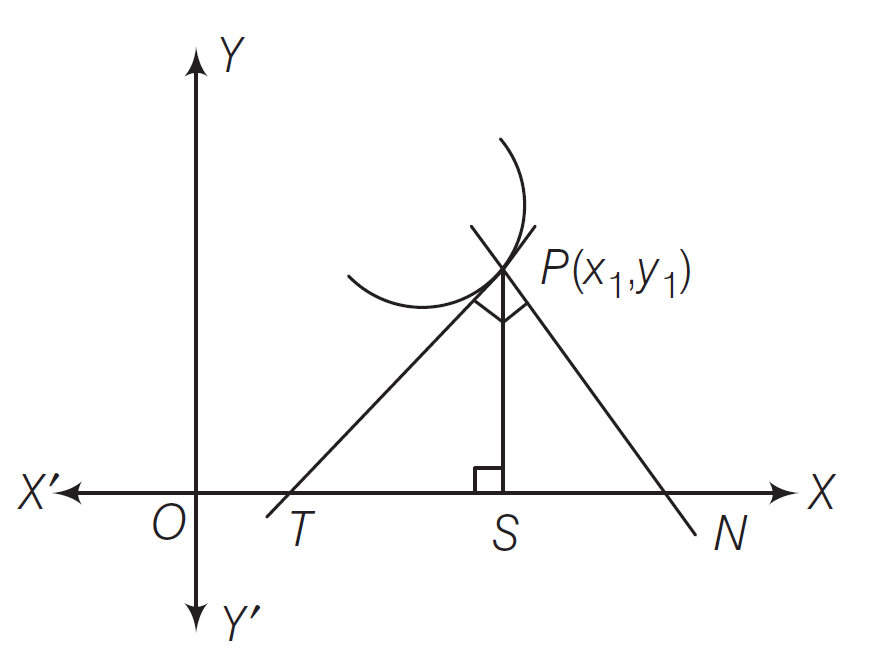
\includegraphics[scale=0.4]{image.png}

\subsection{Length of Tangent}
The portion of the tangent intercepted between the point of contact and $x$ axis.

$$\textbf{Len(Tangent)}=PT=\abs{y_{1}\displaystyle\sqrt{1+\left(\dv{x}{y}\biggr\rvert_{P}\right)^2}}$$

\subsection{Length of Normal}
The portion of the normal intercepted between the point of contact and $x$ axis.

$$\textbf{Len(Normal)}=PN=\abs{y_{1}\displaystyle\sqrt{1+\left(\dv{y}{x} \biggr\rvert_{P}\right)^2}}$$

\subsection{Subtangent}
The projection on the $x$ axis of the Length of Tangent.

$$\textbf{Subtangent}=ST=\abs{y_{1}\cdot \dv{x}{y} \biggr\rvert_{P}}$$

\subsection{Subnormal}
The projection on the $x$ axis of the Length of Normal.

$$\textbf{Subnormal}=SN=\abs{y_{1}\cdot \dv{y}{x} \biggr\rvert_{P}}$$

\section{Rolle's Theorem}
If $f$ is a real-valued function defined on the closed interval $[a,b]$ such that \begin{enumerate}[i.]
    \item $f(x)$ is continuous in the closed interval $[a,b]$
    \item $f(x)$ is differentiable in the open interval $(a,b)$
    \item $f(a)=f(b)$
\end{enumerate} Then, there is at least one value $c$ in $(a,b)$ for which $f'(c)=0$ 

\section{Lagrange's Mean Value Theorem}
\subsection*{First Form}
If a function $f(x)$, \begin{enumerate}[i.]
    \item is continuous in the closed interval $[a,b]$
    \item is differentiable in the open interval $(a,b)$
\end{enumerate} Then, there is at least one value $c \in (a,b)$, such that $$f'(c)=\dfrac{f(b)-f(a)}{b-a}$$
\subsection*{Second Form}
If $b=a+h$, $c=a + \theta h$, where $0<\theta <1 \hfill [a<c<b]$

Then, the mean value theorem can be stated as follows:

If $i. f(x)$ is continuous in the closed interval $[a,a+h]$

$ii. f'(x)$ exists in the open interval $(a,a+h)$, then there exists at least one number $\theta \in (0,1)$, such that $$f(a+h)=f(a)+hf'(a+\theta h)$$

\section{Analysis of Cubic Polynomial}
Let $f(x)=ax^3+bx^2+cx+d$

\begin{itemize}
    \item \textbf{Case I} $f'(x)$ has no Real Root.

    $\implies D<0$ 
    
    $\therefore f(x)=0$ has One Real Root and Two Imaginary Roots.
    \item \textbf{Case II} $f'(x)$ has Two Equal Roots.

    Let the repeated root of $f'(x)$ be $x=\alpha$

    $\implies f'(x)=k\left(x-\alpha\right)^2$

    $\implies f(x)=\dfrac{k\left(x-\alpha\right)^3}{3}+C$

    If $C=0$, $f(x)=0$ has Three Real Equal Roots.

    If $C \not= 0$, $f(x)=0$ has One Real Root and Two Imaginary Roots.
    \item \textbf{Case III} $f'(x)$ has Two Real and Distinct Roots

    Let roots of $f'(x)=0$ be $\alpha, \beta$
    \begin{enumerate}[i.]
        \item $f(\alpha)\cdot f(\beta)>0$

        $f(x)=0$ has One Real and Two Imaginary Roots.

        \item $f(\alpha)f(\beta)<0$

        $f(x)=0$ has Three Real and Distinct Roots.

        \item $f(\alpha)\cdot f(\beta)=0$

        $f(\alpha)=0$ or $f(\beta)=0$

        $f(x)=0$ has Three Real Roots of which Two are equal.

        \item The Graph of every cubic polynomial must have exactly one point of inflection.
    \end{enumerate}
\end{itemize}

\section{Shortest Distance Between Two Curves}
The shortest Distance Between Two Curves always lies along the common normal.
\end{document}